\documentclass[a4paper,11pt]{article}
\usepackage[utf8]{inputenc}
\usepackage[paper=a4paper, hmargin=1.5cm, bottom=1.5cm, top=3.5cm]{geometry}
\usepackage[T1]{fontenc}
\usepackage[spanish]{babel}
\usepackage[colorlinks=true, linkcolor=blue]{hyperref} %Links para el indice.
\usepackage{amsfonts}
\usepackage{verbatim}
\usepackage{listings}
\usepackage{caption}
\usepackage{subcaption}

\usepackage[section]{placeins}
\usepackage{float}
%\usepackage{adjustbox}
\usepackage{amsmath}
\usepackage{blindtext}
\usepackage{sidecap}
\usepackage{color}
\usepackage{graphicx}
\usepackage{algpseudocode}
\usepackage{wrapfig}

\usepackage{algorithm}
\usepackage{algpseudocode}
% \newcommand{\real}{\hbox{\bf R}}

\newcommand{\funcName}[1]{\textbf{\texttt{#1}}}


\title{Trabajo Práctico de Sistemas Operativos}

\begin{document}

\maketitle

\begin{center}
	Universidad de Buenos Aires - Departamento de Computaci\'on - FCEN
\end{center}

\vspace{2cm}
Integrantes:

\begin{itemize}
	\item Castro, Dami\'an L.U.: 326/11  \verb+ltdicai@gmail.com+
	\item Toffoletti, Luis L.U.: 827/11 \verb+luis.toffoletti@gmail.com+
	\item Zanollo, Florencia L.U.: 934/11 \verb+florenciazanollo@gmail.com+
\end{itemize}

\newpage

\tableofcontents

\newpage

\section{Introducción}
Una computadora moderna consiste de uno o m\'as procesadores, memoria, discos, impresoras y uno o varios dispositivos de entrada/salida. Adem\'as una computadora ejecuta programas que suelen intentar acceder a estos recursos y generalmente asumiendo que son los \'unicos que desean utilizarlos. Sin embargo esto casi nunca es cierto y suelen haber conflictos cuando dos procesos (programas en ejecuci\'on) acceden al mismo recurso. Para solucionar estas problem\'aticas se recurre a los sistemas operativos, que son aquellos que se encargan de coordinar el acceso a los recursos por parte de los procesos. Un sistema operativo es un proceso superior a todos los dem\'as y decide, siguiendo alguna normativa, en que momentos los procesos comunes se ejecutan. Se conoce a esta normativa como pol\'itica de \emph{scheduling}, y no hay una \'unica manera de definirla. Dependiendo de la situaci\'on puede que se prefiera pol\'iticas que permitan a los procesos mantener ocupado un recurso durante per\'iodos largos de tiempo mientras que otras pol\'iticas se valen en desalojar a las tareas y otorgarle los recursos a otra tarea. Se espera que un \emph{scheduler} trate de cumplir los siguientes objetivos:

\begin{itemize}
	\item Ecuanimidad (\emph{fairness}): que cada proceso reciba una dosis “justa” de CPU (para alguna definici\'on de justicia).
	\item Eficiencia: tratar de que la CPU est\'e ocupada todo el tiempo.
	\item Carga del sistema: minimizar la cantidad de procesos listos que est\'an esperando CPU.
	\item Tiempo de respuesta: minimizar el tiempo de respuesta percibido por los usuarios interactivos.
	\item Latencia: minimizar el tiempo requerido para que un proceso empiece a dar resultados.
	\item Tiempo de ejecuci\'on: minimizar el tiempo total que le toma a un proceso ejecutar completamente.
	\item Rendimiento (throughput): maximizar el n\'umero de procesos terminados por unidad de tiempo.
	\item Liberaci\'on de recursos: hacer que terminen cuanto antes los procesos que tiene reservados m\'as recursos.
\end{itemize}

Como se puede intuir, es imposible cumplir todos los objetivos a la vez, por lo tanto las pol\'iticas de \emph{scheduling} tienen sus ventajas y sus desventajas. Es el enfoque de este informe exhibir dichas pol\'iticas, su implementaci\'on en lenguaje \emph{C++} y mostraremos sus pros y sus contras con ejemplos.

\subsection{Simulador}

Para analizar las diferentes pol\'iticas de \emph{scheduling} utilizamos un modelo de computadora simplificado que consiste en los siguientes componentes:

\begin{itemize}
	\item Un lote de programas a ejecutar.
	\item Uno o varios n\'ucleos (\emph{cores}) de procesamiento, que se encargar\'an de hacer los c\'omputos de los procesos.
	\item Un \'unico dispositivo de entrada y salida que todos los procesos pueden utilizar si lo desean.
\end{itemize}

\subsubsection{Acciones del simulador}

El simulador provee a los procesos con tres acciones posibles:

\begin{itemize}
	\item $uso\_CPU$(\emph{n}) que indica que el proceso utilizar\'a el CPU durante \emph{n} ciclos de reloj.
	\item $uso\_IO$(\emph{n}) que indica que el proceso utilizar\'a un recurso de entrada/salida durante $n$ ciclos de reloj. Durante este tiempo el proceso no utiliza al procesador, as\'i que el \emph{scheduler} es libre de utilizar ese tiempo en otra tarea.
	\item $return$ que indica que el proceso ya termin\'o su ejecuci\'on. El \emph{scheduler} debe realizar las acciones necesarias para desalojar al proceso.
\end{itemize}

\subsubsection{Definici\'on de \emph{schedulers}}

Un \emph{scheduler} v\'alido ofrece las siguientes funcionalidades:
\begin{itemize}
	\item \funcName{load(pid)}: Carga un proceso con n\'umero de identificaci\'on \funcName{pid}. 
	\item \funcName{unblock(pid)}: Se realiza cuando un proceso con n\'umero de identificaci\'on \funcName{pid} deja de utilizar un recurso de entrada/salida y desea volver a usar el procesador.
	\item \funcName{tick(cpu,motivo)}: Se ejecuta por cada $tick$ del reloj del procesador \funcName{cpu} y el \funcName{motivo} indica que sucedi\'o con el \'ultimo proceso que estaba en ejecuci\'on.
\end{itemize}


\section{Tareas}
\subsection{TaskConsola}

\begin{algorithm}
 \caption{TaskConsola}
 \begin{algorithmic}[1]
 \Procedure{TaskConsola}{$cant\_ bloqueos, bmin, bmax$}
   \State{seteo semilla de random}
   \For{$i\gets 0, cant\_ bloqueos$}
     \State{$random\_ number\gets modulo(rand(),\ bmax - bmin + 1) + bmin$}\Comment{[1]}
     \State{$Uso\_ IO(random\_ number)$}    
   \EndFor
 \EndProcedure
 \end{algorithmic}
\end{algorithm}

[1]: rand() retorna un número arbitrariamente grande.
Tomando su módulo en (bmax - bmin + 1) nos aseguramos que esté entre 0 y (bmax - bmin).\newline
Luego sumamos bmin, resultando un número entre bmin y bmax.

\section{Pol\'iticas de \emph{scheduling}}
\subsection{First-Come First-Served (FCFS)}

FCFS (First-Come First-Served) un scheduler simple en el cual los procesos son asignados al CPU en el orden en que estos lo requieren.

\begin{wrapfigure}{l}{0.3\textwidth}
  \vspace{-30pt}
  \begin{center}
    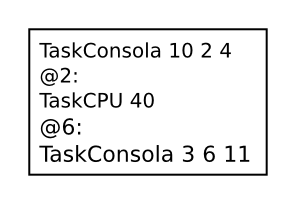
\includegraphics[width=0.25\textwidth]{./FCFS/FCFS_loteTareas.png}
  \end{center}
   \vspace{-30pt}
\end{wrapfigure}

Básicamente hay una sola cola (FIFO) de procesos 'Ready'. 
Cuando un proceso requiere CPU y éste está libre, se lo deja correr tanto tiempo como quiera y sin interrupciones.

A continuación se muestran los gráficos para 1, 2 y 3 núcleos, usando SchedFCFS para el lote de tareas del cuadro.

\vspace{10pt}
\textbf{1 Núcleo:}
\vspace{-20pt}
\begin{center}
 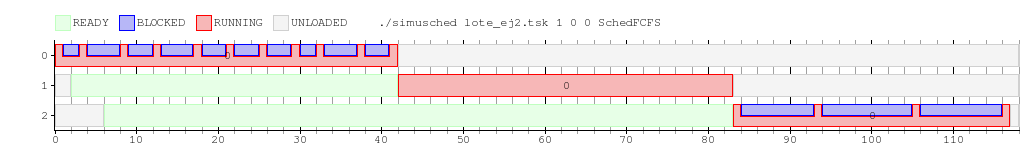
\includegraphics[scale=0.45]{./FCFS/FCFS_1core.png}
\end{center}

\vspace{10pt}

\textbf{2 Núcleos:}
\vspace{-20pt}
\begin{center}
 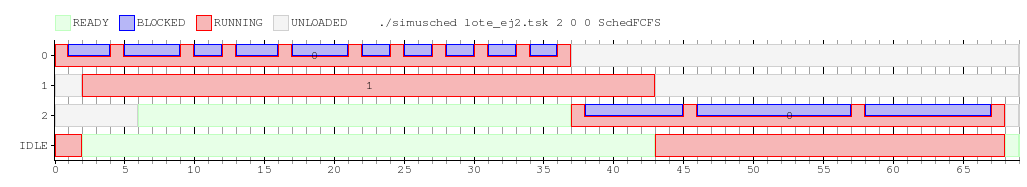
\includegraphics[scale=0.45]{./FCFS/FCFS_2core.png}
\end{center}

\vspace{10pt}

\textbf{3 Núcleos:}
\vspace{-20pt}
\begin{center}
 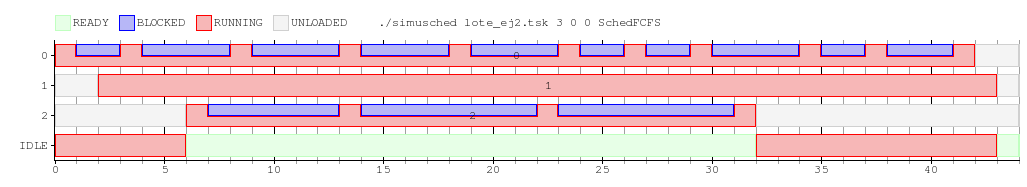
\includegraphics[scale=0.45]{./FCFS/FCFS_3core.png}
\end{center}


Obs: Los parámetros de costo de cambio de contexto y migración fueron seteados en 0 ya que en este scheduler en particular
no son tomados en cuenta. Porque núnca se desalojan las tareas ni se cambian de núcleo.

En los gráficos se hace evidente que a más cántidad de núcleos, mejor rendimiento.
Esto se debe a que FCFS no soporta múltitarea por sí sólo (ya que núnca desaloja a las tareas), sino que necesita varios núcleos para lograrlo.

Las desventajas de FCFS son varias:

\begin{itemize}
\item Como ya dijimos, no soporta múltitarea.
\item Puede generar mucho 'waiting time'.
	Si está ejecutando tareas muy largas las nuevas no entran hasta que éstas terminen.
\item No tiene buen rendimiento, a menos que se sepa la duración de las tareas de antemano.
\item Carece de 'fairness' i.e. no distribuye el/los procesador/es de forma justa entre las tareas.
\end{itemize}
\subsection{Round-Robin (RR)}
RR es un algoritmo de los más viejos, simple, justo y ampliamente usado.

A cada proceso se le asigna un tiempo (quantum) durante el cuál le es permitido correr.
Si el proceso sigue corriendo al final del quantum, los recursos le son quitados y se le da paso a otro proceso.
Si el proceso se bloquea, pierde el quantum que le quedaba y los recursos son dados a otro proceso.

Implementar RR es simple, sólo se requiere una lista de procesos 'Ready'.
Cuando el proceso usa su quantum es puesto al final de la lista. 
Si éste se bloquea, es removido de dicha lista y volverá a ser agregado en cuanto se desbloquee.

En nuestro caso usamos las siguientes estructuras de datos:
 \begin{description}
  \item[Cola de procesos 'Ready']{}
 \end{description}

\begin{algorithm}
 \caption{Round-Robin}
 \begin{algorithmic}[1] 
 \Procedure{load}{$pid$}
   \State{encolo la nueva tarea en readyTasks}
 \EndProcedure


 \Procedure{unblock}{$pid$}
   \State{encolo la tarea desbloqueada en readyTasks}
 \EndProcedure


 \Procedure{tick}{$cpu,\ motivo$}
   \If{el cpu esta ejecutando IDLE}
      \State{llamo a NEXT(cpu) para obtener la próxima tarea a ejecutar}
   \Else
      \If{el motivo es un TICK}
	 \State{Actualizo el quantum}
	 \If{se termino el quantum}
	    \State{encolo la tarea en readyTasks}
	    \State{renuevo el quantum}
	    \State{llamo a NEXT(cpu) para obtener la próxima tarea a ejecutar}
	 \EndIf	    
      \ElsIf{el motivo es un BLOCK o un EXIT}
	  \State{renuevo el quantum}
	  \State{llamo a NEXT(cpu) para obtener la próxima tarea a ejecutar}	
      \EndIf
   \EndIf
 \EndProcedure

 
 \Procedure{next}{$cpu$}
    \If{hay tareas esperando en readyTasks}
	\State{retornar la primera de la cola readyTasks y quitarla}
    \Else
	\State{retornar IDLE}
    \EndIf
 \EndProcedure
 \end{algorithmic}
\end{algorithm}

Para las simulaciones mantuvimos los siguientes costos:
\begin{description}
 \item[costo de cambio de contexto = 1 :]{En un CPU real se deben intercambiar estructuras de datos que contienen información de los procesos antes de poder correr la nueva tarea.}
 \item[costo de migración de núcleo = 2 :]{Se deben intercambiar las mismas estructuras de datos que para el cambio de contexto pero la 'distancia' del caché de un núcleo al de otro es mayor que dentro de sí mismo.}
\end{description}

Correremos un par de lotes de tareas para verificar que el comportamiento del scheduler es el esperado.

\begin{center}
 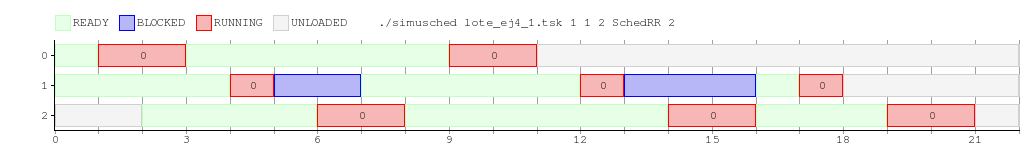
\includegraphics[scale=0.48]{./RR/RR_simple.png}
\end{center}

Se puede observar que no es un algoritmo FCFS porque, en principio, hace desalojo de tareas cada cierto quantum.
Además las tareas que se bloquean son desalojadas de inmediato, sin encolarlas en ReadyTasks hasta que se desbloqueen.

\begin{center}
 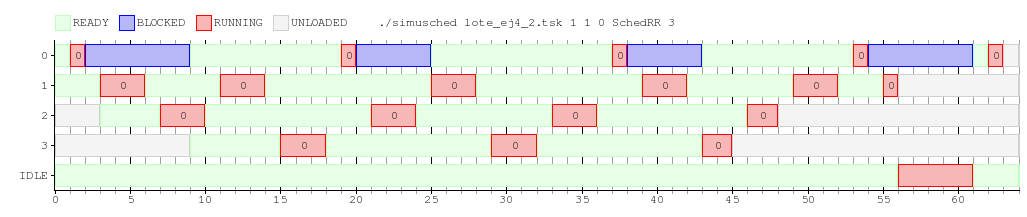
\includegraphics[scale=0.48]{./RR/RR_example_2.png}
\end{center}

Se puede ver que el proceso 0 es desalojado en cuanto se bloquea, cediendo el procesador al
proceso 1 (siguiente en la cola de ReadyTasks).\\
En cuanto el proceso 1 termina su quantum es desalojado (y movido al final de la cola de ReadyTasks).
Y se deja correr el proceso 2.\\

Entre los ciclos 14 y 15, la cola de ReadyTasks tiene la siguiente forma:
[3, 2, 0, 1].\\
Ya que el proceso 0 fue desencolado en cuanto se bloqueó, y vuelto a encolar en el
ciclo 11 (cuando se desbloquea), antes de que termine el quantum del proceso 1.\\

Veamos ahora un ejemplo de una mala elección de quantum para un entorno donde el
costo de cambio de contexto es elevado.

\begin{center}
 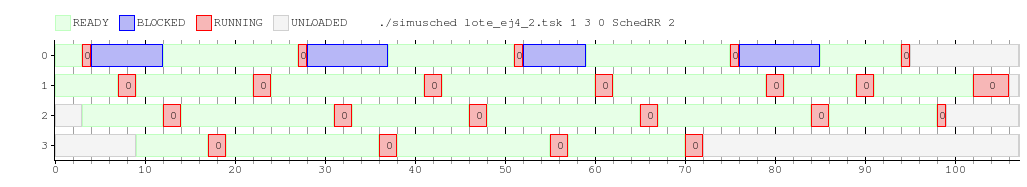
\includegraphics[scale=0.48]{./RR/RR_example_3.png}
\end{center}

Como se puede observar, tarda 106 ciclos en completar la ejecución del lote de tareas.
A diferencia del anterior (que tardaba 63 ciclos).

Esto se debe a que el procesador está más tiempo haciendo tareas de mantenimiento (cambio de contexto)
que efectivamente ejecutando procesos.

\section{Discusi\'on}

\section{Conclusiones}


\end{document}
